\section{Blockschaltbild des Projekts}\label{sec:3.1}
Nach einigen Überlegungen über die beste Herangehensweise an dieses Projekt wurde folgendes Blockschaltbild entwickelt:
\begin{figure} [H]
	\centering
	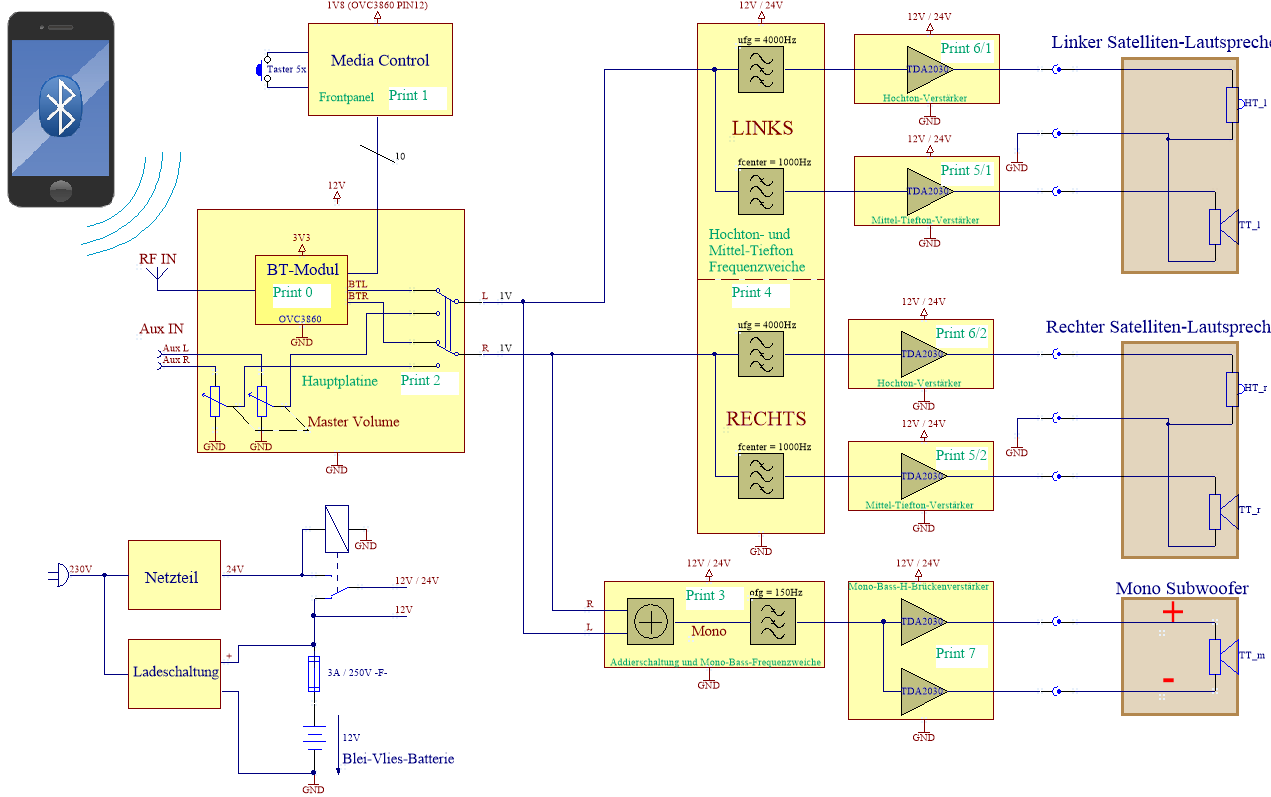
\includegraphics[width=1\textwidth]{img/blockschaltbildV2.png}
	\caption{Blockschaltbild}
	\label{fig:3.1.1}
\end{figure}
Ein wichtiger Teil des Projekts ist die Bluetooth-Hauptplatine (in Abb. \ref{fig:3.1.1} links unten).
Diese Platine verfügt über die Audio-Eingänge des Projekts.
Das Stereo-Audio-Signal kann mithilfe der BT-Hauptplatine mittels Klinkenbuchse oder Übertragung über Bluetooth (siehe: Kap. \ref{sec:3.3}) in die gesamte Schaltung eingespeist werden.
\\ \\
Dieses Stereo-Audio-Signal wird dann mithilfe der Frequenzweichen in 3 verschiedene Frequenzbereiche (Hochton-, Mittel-Tiefton- und Bassbereich) aufgetrennt.
\\
Tiefe Frequenzen (<150Hz) werden \enquote{L + R} (Stereo) addiert und über eine Mono-Tiefpass-Weiche gefiltert.
\\
Insgesamt gibt es dann also 5 Signale, die weiterverarbeitet werden:
\\ 
\begin{itemize}
	\item Hochton-Links
	\item Hochton-Rechts
	\item Mittel-Tiefton-Links
	\item Mittel-Tiefton-Rechts
	\item Mono-Bassbereich
\end{itemize}

Die verschiedenen Audio-Signale werden dann mit je einem Leistungs-Verstärker auf einen höheren Pegel gebracht.
Die Ausgangsleistung der Leistungs-Verstärker variiert je nach Frequenzbereich.
Dies ist bedingt durch die verwendete Verstärkerschaltung.\\
Diese Schaltungen sind für:
\begin{itemize}
	\item \textbf{Hochtonbereich:}\\ TDA2030-Leistungsverstärker-Grundschaltung
	\item \textbf{Mittel-Tieftonbereich:}\\ TDA2030-Leistungsverstärker erweitert mit Leistungstransistoren
	\item \textbf{Bassbereich:}\\ TDA2030-Leistungsverstärker erweitert mit Leistungstransistoren in H-Brücke geschallten
\end{itemize}
Aus diesen Schaltungen erschließen sich folgende maximale Ausgangsleistungen bei asymmetrischer Spannungsversorgung von 24V und 1\% Klirrfaktor:\\
\begin{itemize}
	\item Hochton-Leistungsverstärker (an 8 Ohm): 6W
	\item Mittel-Tiefton-Leistungsverstärker (an 4 Ohm): 11W
	\item Bassbereich-Leistungsverstärker (an 4 Ohm): 44W
\end{itemize}

Versorgt wird die Elektronik unter Akkubetrieb mit 12 V oder 24 V unter Netzbetrieb, genauere Erklärung im Kapitel \ref{sec:3.4}.
Somit sind die Leistungs-Verstärker-Schaltungen noch nicht stark ausgelastet, da diese für maximal \enquote{+/- 22V} oder \enquote{+ 44V asymmetrisch} ausgelegt sind.

%Da eine Blei-Vlies-Batterie für das Projekt vorgesehen war und diese zumeist 12V liefern, ist die Entscheidung von einer 12V Spannungsversorgung sehr nahe.
%Andere Alternativen wie zB. LiPo-Akkus könnten mehr Spannung und Strom liefern, diese sind jedoch um einiges vorsichtiger zu Behandeln (sehr hohe Energiedichte) und daher auch umständlicher (Lade-Überwachung, Brandgefahr).

\newpage
\section{Mehrweg-Lautsprechersysteme}\label{sec:3.2}
Ein Lautsprecher ist ein Bauelement, das ein elektrisches Signal in ein akustisches Signal (20 Hz bis 20 kHz) umwandelt.
Dabei wird eine Membran in Schwingung versetzt, die wiederum die umgebende Luft zum Schwingen bringt und einen hörbaren Ton erzeugt.
\\ \\
Nun wird aber nicht jede Frequenz gleich gut von ein und demselben Lautsprecher abgestrahlt.
Durch die physikalischen Gegebenheiten strahlen große Membranen tiefe Frequenzen besser ab als hohe Frequenzen.
In der Abbildung \ref{fig:3.2.1} wird der Audiobereich in drei Bereiche aufgeteilt, was auch der jeweiligen Lautsprecher-Charakteristik entspricht.\\
Kennlinienbeschriftung:\\
\begin{itemize}
	\item \textbf{Hochton-Bereich}: Rot
	\item \textbf{Mittel-Tiefton-Bereich}: Grün
	\item \textbf{Tiefton(Bass)-Bereich}: Dunkelblau
	\item \textbf{Summe der Bereiche}: Schwarz	
\end{itemize}
Es ist sinnvoll, mehrere Lautsprecher für verschiedene Frequenzbereiche zu verwenden.
Benannt werden diese verschiedenen Lautsprecher durch den Bereich, in dem sie am besten funktionieren.
Beispielsweise Hochton-Lautsprecher oder Hochtöner für den Hochton-Bereich (>2,5 kHz).
Wie gut nun verschiedene Frequenzen von einem Lautsprecher abgestrahlt werden, ist in seinem Frequenzgang ersichtlich:
\begin{figure} [H]
	\centering
	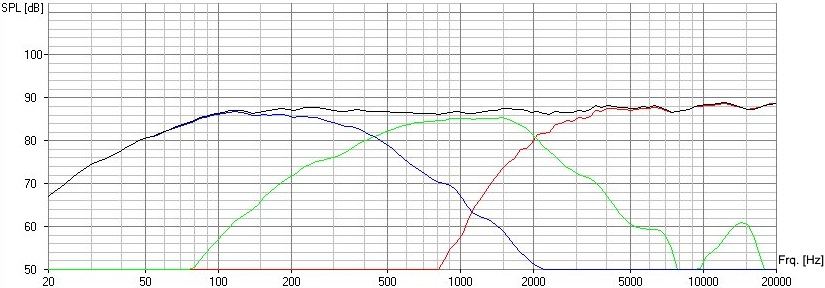
\includegraphics[width=1\textwidth]{img/Grundlagen/Mehrweg-Lautsprechersysteme/Frequenzbereiche-Audio-cut.jpg}
	\caption{Tiefton-, Mittelton- und Hochton-Bereich\\- (Beispiel eines Lautsprecher-Systems)}
	\label{fig:3.2.1}
\end{figure}
\footnotetext{http://http://www.lavalu.de/images/Frequenzgang.jpg\\Zugriff: 23.03.2017}

Bei einem perfekten Lautsprecher würde diese Linie bei 20 Hz beginnend (Abb. \ref{fig:3.2.1}) eine parallele Gerade zur X-Achse bilden, bis hin zu 20 kHz.
Da so ein Lautsprecher nur eine ideale Annahme und nicht realisierbar ist, werden in der Praxis mehrere Lautsprecher zusammen verwendet, um sich an dieses Ideal anzunähern.
Wie in der Abbildung \ref{fig:3.2.1} gut ersichtlich, ergeben die einzelnen Frequenzgänge der Lautsprecher aufsummiert den gesamt Frequenzverhalten des Systems (in Schwarz), der relativ linear ist.
Unterhalb von 100 Hz ist zwar noch eine größere Pegel-Lücke, die aber durch einen besseren Subwoofer ausgebessert werden kann.

\subsubsection*{Frequenzweichen in Zusammenhang mit Lautsprechersystemen}
Das Diagramm (Abb. \ref{fig:3.2.2}) stellt ein Beispiel für die Übertragungskennlinien von Frequenzweichen dar.
In diesem sind die Eigenschaften der jeweiligen Filterarten gut ersichtlich (Siehe auch \ref{sec:8.4}).\\
Betrachtet man nur die dunkelblaue Kurve ist sofort ersichtlich, dass über 400 Hz der Pegel stark abnimmt bis hin zu 0.
Dies ist auch ersichtlich bei der grünen Kurve.
Bei dieser strebt der Pegel unter 400 Hz und oberhalb 2 kHz gegen Null.
In der roten Kurve hingegen ist der Frequenzbereich von unter 2 kHz geringer, bzw. nicht vorhanden.
\\
Es sind klare Schnittpunkte der Kurven ersichtlich, welche auch bewusst gewählt sind.
Diese Übertragungskennlinien der Frequenzweichen sind für ein 3-Weg-System optimiert, d.h. das Eingangssignal wird, durch die entsprechenden Weichen, auf drei Teile aufgeteilt.
Die Übertragungskennlinien, und somit die Schnittpunkte, variieren von System zu System.\\
Nach der Auftrennung wird jedes Teilsignal mit einem jeweils eigenen Verstärker verstärkt.
%Da so ein Lautsprecher aber nicht existiert, werden verschiedene Frequenzen auch mit einem verschiedenen Schalldruckpegel vom Lautsprecher abgestrahlt.
\begin{figure} [H]
	\centering
	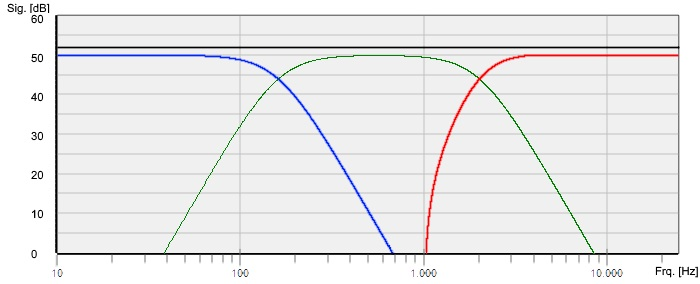
\includegraphics[width=0.8\textwidth]{img/Grundlagen/Mehrweg-Lautsprechersysteme/Frequenzbereiche-Audio-Weiche-cut.jpg}
	\caption{Tiefpass-, Bandpass- und Hochpass-Weiche - (Beispiel für das Verhalten von Frequenzweichen)}
	\label{fig:3.2.2}
\end{figure}
\footnotetext{http://www.audiovero.de/acourate-wiki/lib/exe/fetch.php?media=bilder\_funktionen:funkt\_bsp\\\_addition\_02.png\\Zugriff: 23.03.2017}

Diese Schnittstellen können durch Verändern der Grenzfrequenzen der Frequenzweichen beeinflusst werden.
Die Höhe des Pegels kann durch in der Schaltung verbaute Trimmpotentiometer verändern werden.
Somit können die Pegel der verschiedenen Lautsprecher untereinander angepasst werden um einen gleich hohen Pegel an allen Lautsprechern zu erreichen.
Ohne diese Anpassung werden bestimmte Frequenzen lauter wiedergegeben als andere, was wieder einen nichtlinearen Frequenzgang bedeuten würde.\\ \\

%\newpage
\subsubsection*{Allgemeines zu Lautsprecher-Systemen}
Je nach Frequenzbereich kann ein Ton vom menschlichen Ohr lokalisiert \mbox{werden} oder nicht.
Hohe Frequenzen (>1 kHz) sind besser lokalisierbar als tiefe Frequenzen.
Bei sehr niedrigen Frequenzen (<80 Hz) ist der Ton gar nicht mehr lokalisierbar. % Aus Wikipedia <80Hz!
Das kann man nutzen und damit akustische Effekte erzeugen.
Einige Lautsprecher-Systeme, die diesen Effekt nutzen sind:
\begin{itemize}
	\item 2.0 - System
	\item 2.1 - System
	\item 5.1 - System
\end{itemize}
Dabei steht die erste Ziffer für die Anzahl der verteilten Lautsprecher und die zweite Ziffer für die Anzahl der verwendeten Subwoofer.
\\
Je mehr verteilte Lautsprecher (auch Satelliten genannt) benutzt werden, desto bessere Raumklang-Effekte sind realisierbar.
Dadurch wird die Beschaltung aber auch komplizierter, da zB. 5+1 verschiedene Audio-Signale verwendet werden.
\\ \\
Der Subwoofer ist ein spezieller Lautsprecher.
Er arbeitet im Bass-Bereich(20 bis 150 Hz).
Diese Frequenzen sind nicht lokalisierbar, weshalb auch nur ein Subwoofer benötigt wird.
Meistens ist die Membran des Subwoofers um einiges größer als die Membran anderer Lautsprecher.
Damit kann der Subwoofer mehr Luft in Bewegung setzen und somit einen höheren Schalldruckpegel erzeugen.
Um das zu ermöglichen benötigt der Subwoofer aber auch mehr Leistung als ein Lautsprecher für einen anderen Frequenzbereich.
\\ \\

\newpage
\subsection*{Zu den Verschiedenen Lautsprecher-Systemen:}
\subsubsection*{2.0 - System}
\begin{figure} [H]
	\centering
	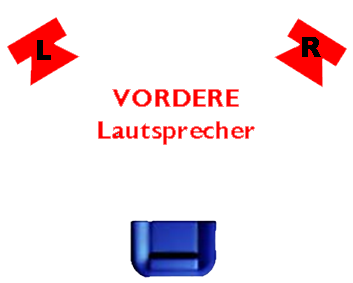
\includegraphics[width=0.5\textwidth]{img/Grundlagen/Mehrweg-Lautsprechersysteme/DOLBYDigital20-cut.jpg}
	\caption{2.0-Lautsprecher-System}
	\label{fig:3.2.3}
\end{figure}
\footnotetext{Editiert:\enquote{https://upload.wikimedia.org/wikipedia/commons/6/62/DOLBY\_Digital\_5.1.png}\\Zugriff: 23.03.2017}

Dieses System, bestehend aus linker und rechter Lautsprecherbox (Abb. \ref{fig:3.2.3}), eignet sich bereits für Stereo-Klang.
Meistens beinhalten diese Boxen einen Hochton-Lautsprecher und einen Tiefton-Lautsprecher.
Diese müssen eine entsprechende Qualität aufweisen, um ohne Mittelton-Lautsprecher auszukommen.\\
Eine Variante mit drei verschiedenen verbauten Lautsprecher-Chassis für jeden Frequenzbereich, ist auch üblich.
Der Vorteil dieser Bauart ist, dass die Lautsprecher-Chassis einen geringeren Bereich mit einem linearen Frequenzgang abdecken müssen und daher zumeist von geringerer Qualität sein können.\\
Bei der Ausrichtung dieser Lautsprecher ist zu beachten:
\begin{enumerate}
	\item Die Lautsprecher-Chassis sollen in Richtung des Testers zeigen
	\item Die Hochton-Lautsprecher sollen sich auf Ohrenhöhe des Testers befinden
	\item Die Lautsprecher-Boxen sollen optimaler weise, wie eingezeichnet, einen 30° Winkel zur Blickrichtung des Testers aufweisen
\end{enumerate}
Die Hochton-Lautsprecher müssen sich aus diesem Grund auf Ohrenhöhe befinden, da sich hohe Frequenzen geradliniger ausbreiten als tiefe und man sie somit besser wahrnehmen kann.
%Um einen optimalen Klang zu erhalten, müssen sich diese deshalb auf Höhe der Ohren befinden, um diese geradlinige Ausbreitung direkt wahrzunehmen.\\

\begin{figure} [H]
	\centering
	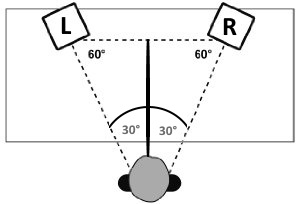
\includegraphics[width=0.5\textwidth]{img/Grundlagen/Mehrweg-Lautsprechersysteme/opt-20-aufstellung.jpg}
	\caption{Optimale Ausrichtung zum Tester}
	\label{fig:3.2.4}
\end{figure}
\footnotetext{Editiert:{https://images-eu.ssl-images-amazon.com/images/G/03/electronics/aplus/B0059DM2F\\E.001.\_SL300\_.jpg}\\Zugriff: 24.03.2017}

Für dieses System wird mindestens eine Aufteilung in zwei Audio-Signale benötigt (links und rechts).\\
Wie bereits erwähnt, wird auch ein Tiefton-Lautsprecher verbaut.
Dieser gilt aber nicht als Subwoofer aus folgenden Gründen:
\begin{enumerate}
	\item Es ist in der Lautsprecher-Box auch ein Lautsprecher-Chassis für andere Frequenzbereiche verbaut
	\item Der Tiefton-Lautsprecher strahlt nicht nur den nicht-lokalisierbaren Frequenzbereich ab
\end{enumerate}
Da das Lautsprecher-System aus 2 verteilten Boxen und keinem Subwoofer besteht nennt man das Lautsprecher-System ein \enquote{2.0 - System}.


\newpage
\subsubsection*{2.1 - System}
\begin{figure} [H]
	\centering
	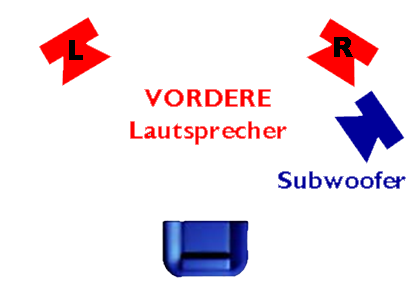
\includegraphics[width=0.5\textwidth]{img/Grundlagen/Mehrweg-Lautsprechersysteme/DOLBYDigital21-cut.jpg}
	\caption{2.1-Lautsprecher-System}
	\label{fig:3.2.5}
\end{figure}
\footnotetext{Editiert:\enquote{https://upload.wikimedia.org/wikipedia/commons/6/62/DOLBY\_Digital\_5.1.jpg}\\Zugriff: 23.03.2017}

Dieses System besteht aus 2 + 1 Lautsprecher-Boxen, und zwar eine linken und rechten Satelliten-Box und einer Subwoofer-Box.
Hier ist wiederum Stereo-Klang möglich, nun aber mit Unterstützung für den Bass-Bereich (<150 Hz).
Die Anordnung der Satelliten ist vorgegeben (links und rechts).
Die Subwoofer-Box darf im Raum verstellt werden, da wie bereits erklärt die abgestrahlten Frequenzen des Subwoofers schwer bzw. nicht lokalisierbar sind.\\
Für dieses System wird die Aufteilung in mindestens 3 Audio-Signale benötigt:
links, rechts, Bass-Bereich.\\
Für die meisten allgemeinen Konsumenten-Anwendungen wird ein 2.1-System verwendet.\\ 
Es ist üblich, dass in den Satelliten-Boxen wieder zwei Lautsprecher-Chassis verbaut werden.
Eines für den Hochton- und eines für den Mittel-Tiefton-Bereich.
In diesem Fall muss der Mittel-Tiefton-Lautsprecher die sehr tiefen Frequenzen nicht übernehmen, das macht der Subwoofer.
Somit ergibt sich eine Aufteilung des Frequenzbereiches auf drei Lautsprecher, was wiederum bedeutet, dass diese in einem geringeren Frequenzbereich linear arbeiten müssen.\\
Wenn ein guter Mittel-Tiefton-Lautsprecher verwendet wird der einen annähernd linearen Frequenzgang bis in den Hochton-Bereich aufweist, kann man auch einen schlechteren Hochton-Lautsprecher in Kombination mit diesem verwenden.\\
Eine billigere Variante würde die Ausführung der Satelliten-Boxen mit jeweils einem Breitband-Lautsprecher bieten.\\
Da der Subwoofer nur einen sehr geringen Teil des Frequenzgangs übernimmt (20...150 Hz), werden trotzdem relativ gute Lautsprecher-Chassis für Mittel-Tiefton- und Hochton-Bereich benötigt.



\subsubsection*{5.1 - System}
\begin{figure} [H]
	\centering
	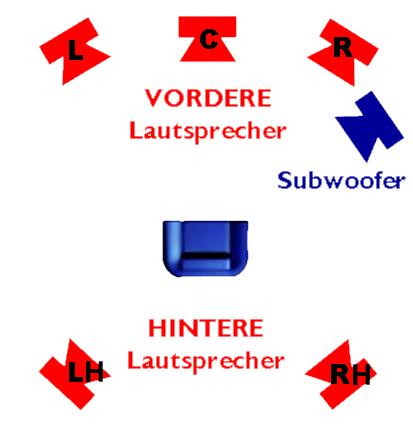
\includegraphics[width=0.5\textwidth]{img/Grundlagen/Mehrweg-Lautsprechersysteme/DOLBYDigital51-cut.jpg}
	\caption{5.1-Lautsprecher-System}
	\label{fig:3.2.6}
\end{figure}
\footnotetext{Editiert:\enquote{https://upload.wikimedia.org/wikipedia/commons/6/62/DOLBY\_Digital\_5.1.png}\\Zugriff: 23.03.2017}

Dieses System besteht aus 5+1 Lautsprecher-Boxen:
\begin{itemize}
	\item \textbf{L}inks-Vorne
	\item \textbf{C}enter
	\item \textbf{R}echts-Vorne
	\item \textbf{L}inks-\textbf{H}inten
	\item \textbf{R}echts-\textbf{H}inten
	\item Subwoofer
\end{itemize}
Mit diesem System ist ein sogenannter \enquote{Surround-Sound} möglich.
Das bedeutet, dass der Tester inmitten dieses Systems rundum beschallt wird.
Die Anordnung bis auf die des Subwoofers ist wieder vorgegeben.
Für dieses System wird die Aufteilung in mindestens 6 Audio-Signale benötigt.
Diese werden entsprechend den zuvor genannten Lautsprecher-Boxen benannt.\\
Der \enquote{Center}-Lautsprecher ist aus diesem Grund wichtig da sich aus der Erfahrung heraus bewiesen hat, dass Sprache von einem Menschen, der bei einem Film sich in mitten des Bildes befindet, sich akustisch mittig lokalisieren lassen sollte.\\ 
Ein solches System kann man oft in Heimkinos finden.
Kinosäle besitzen meistens noch besser ausgeklügelte, bzw. größere Systeme.
\\ \\


In unserem Projekt haben wir uns für ein 2.1 - System entschieden, da sich dieses System am besten bewährt hat und für Musik ein Stereo-System mit Mono-Subwoofer völlig ausreicht.
Die zwei Satelliten-Lautsprecher sind mit je einem Hochton- und einem Tiefton-Lautsprecher ausgestattet und werden über Audio-Kabel mit der Hauptbox verbunden.
Damit sollen die Satelliten-Lautsprecher fast den gesamten Frequenzbereich für Audio (20 Hz bis 20 kHz) abdecken.
Der einzelne Subwoofer übernimmt den Bass-Bereich (<150 Hz) und sitzt in der Hauptbox.
Dort ist auch die gesamte Elektronik verbaut.


\newpage
\section{Signalübertragung über Bluetooth}\label{sec:3.3}
Bluetooth ist eine moderne Funkschnittstelle für verschiedenste Anwendungen.
Unter anderem gibt es auch speziell für Audio-Anwendungen konzipierte Protokolle.
Die Übertragung läuft folgendermaßen ab:
\\
Zuerst muss das sendende Gerät (z.B. ein Smartphone) mit dem empfangenden Gerät (z.B. Bluetooth-Modul) verbunden werden.
Danach werden die gewünschten Daten ausgewählt.
In diesem Fall sind die Daten ein Musikstück.
Über Funk werden die digitalen Daten an das empfangende Gerät gesendet.
Nun muss das Bluetooth-Modul diese digitalen Daten wieder in ein analoges Signal umwandeln, welches dann weiterverarbeitet werden kann.
\\ \\
Dabei ist eine hohe Kompatibilität mit viele Geräten wichtig, weil es sehr viele verschiedene Versionen von Bluetooth gibt.
Da Bluetooth-Geräte meist abwärtskompatibel sind, ist es sinnvoll das Modul mit einer älteren BT-Version laufen zu lassen.
\\ \\
Nach ausführlicher Recherche wurde das Modul \enquote{XS3868} ausgewählt.
Der darauf verbaute Chip \enquote{OVC3860} von \enquote{OmniVision Technologies} hat sich bereits in vielen anderen Projekten bewährt, da er günstig ist und Funktionen wie \enquote{Play/Pause} bereitstellt.

\begin{figure} [H]
	\centering
	
\includegraphics[width=1\textwidth]{img/Grundlagen/Bluetooth/BT-uebertragung-cut.jpg}
	\caption{Bluetooth-Funkübertragung - Schematisch}
	\label{fig:3.3.1}
\end{figure}
\footnotetext{Editiert:\enquote{http://themetro.de/wp-content/uploads/bluetooth\_mac\_artikelbild.png \\http://icon-icons.com/icons2/875/PNG/512/big-music-player-speaker\_icon-icons.com\_68248.png }\\Zugriff: 24.03.2017}



\newpage
Im \enquote{OVC3860} (Abb. \ref {fig:3.3.2}) ist außer der Bluetooth-Verbindung auch noch ein Stereo-Audio-Prozessor verbaut.
Zusätzlich gibt es noch eine UART-Schnittstelle, mit deren Hilfe man einige Einstellungen am Chip vornehmen kann.
Eine LiPo-Akku-Ladeschaltung ist ebenfalls vorhanden, wird aber in diesem Projekt nicht verwendet.
\\
Das Modul benötigt eine Versorgungsspannung von 3,3 V bis 4,2 V, wobei der Chip mit 1,8 V versorgt wird.
Diese Spannung (1,8 V) wird auf dem Modul erzeugt.
\\
Die verwendete BT-Version ist 2.0.
Einige GPIO-Pins sind auf das Modul herausgeführt, um Funktionen wie \enquote{Play/Pause} zu ermöglichen.
Der Chip benötigt einen externen Speicher und eine Antenne (auf dem Modul) um ordnungsgemäß zu funktionieren.
\begin{figure} [H]
	\centering
	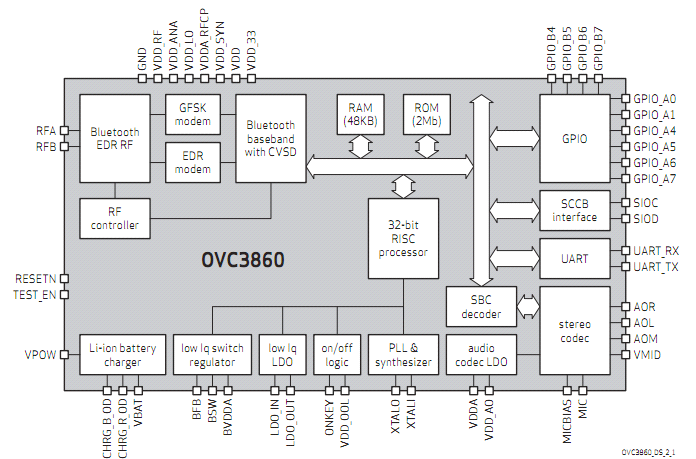
\includegraphics[width=1\textwidth]{img/BTModul/blockschaltbild.png}
	\caption[Blockschaltbild OVC3860]{Blockschaltbild OVC3860\footnotemark}\label {fig:3.3.2}
\end{figure}
\footnotetext{http://cxem.net/review/files/review24\_OVC3860.pdf,\\Zugriff: 11.03.2017}

\newpage
\section{Spannungsversorgung}\label{sec:3.4}
Die gesamte Box soll portabel sein, d.h. auch ohne externe Stromzufuhr funktionieren.
Dafür ist ein Akku notwendig.
Nach einigen Überlegungen haben wir uns für einen Blei-Vlies-Akku entschieden.
Gründe dafür sind:
\begin{itemize}
	\item Geringe Kosten
	\item Einfache Beschaltung
	\item Geringere Gefahr gegenüber Lithium-Akkus
	\item Vlies-Technik: Kein Auslaufen von chemischen Substanzen
\end{itemize}
Dieser Akku versorgt die Elektronik mit 12 V (DC) und wird über ein passendes Ladegerät aufgeladen.
Da aber mit dieser relativ geringen Spannung nur eher kleine Leistungen zu erwarten sind, kam die Idee auf, die Verstärker und Weichen bei externer Versorgung durch das Stromnetz (230 V / AC) mit einer größeren Spannung (24 V / DC) zu versorgen.
Um das zu realisieren wird ein Netzteil, in unserem Fall ein Schaltnetzteil, benötigt.
Falls das Gerät am externen Stromnetz hängt, wird die Versorgung der Verstärker automatisch mithilfe eines passenden Relais umgeschaltet.
Diese Lösung wurde gewählt, da sie sehr simpel ist und gut funktioniert.
Veranschaulicht wird das Konzept durch diese Schaltung:
\begin{figure} [H]
	\centering	
	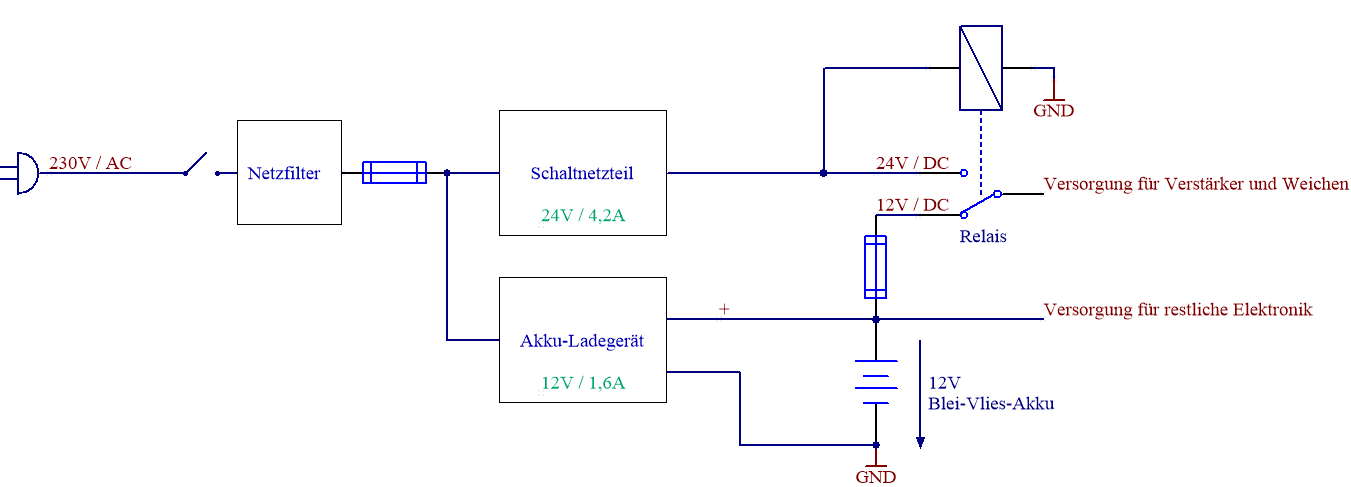
\includegraphics[width=1\textwidth]{img/Grundlagen/VersorgungV2.png}
	\caption{Versorgungskonzept}
	\label {fig:3.4.1}
\end{figure}
Das Lautsprecher-System kann somit bei Netzbetrieb die Musik lauter abspielen als bei Akku-Betrieb.

% ANDERE VERSION
%Da das Projekt portabel sein soll, ist auch ein Akku (Vlies-Blei-Akku) eingebaut.
%Er versorgt die gesamte Elektronik mit 12 V bei Akkubetrieb.
%Aufgeladen wird er durch ein passendes Ladegerät, welches aber nicht von uns entwickelt wird.
%\\ \\
%Falls eine externe Stromversorgung über eine Steckdose (230V AC) gegeben ist, ändert sich die Versorgung der Verstärker.
%Während nun der Akku aufgeladen wird, schaltet ein Relais die Versorgungsspannung der Verstärker von 12 V auf 24 V um.
%Diese Spannung (24 V) wird durch ein Schaltnetzteil erzeugt.
%\\ \\
%Durch eine höhere Spannung können die Verstärker auch die Signale auf höhere Spannungen verstärken.
%Somit ergibt sich eine höhere Leistung an den Verstärkern aber auch an den Lautsprechern.
%Eine Leistungssteigerung an einem Lautsprecher entspricht einer Steigerung des Schalldruckpegels was wiederum eine höhere Lautstärke bewirkt.
%An den Verstärkern bewirkt eine höhere Leistung auch eine größere Wärmeentwicklung.
%Der verbaute Kühlkörper muss diese Wärme bei Akkubetrieb als auch bei Netzbetrieb ableiten können.
%\\ \\
%Das Lautsprecher-System kann somit bei Netzbetrieb die Musik lauter abspielen, als bei Akku-Betrieb.
